\chapter{Overview}
\label{chap:overview}

The primary goal of \iqd{} is to provide a scalable architecture for executing incremental queries over large models. Our approach is based on the following foundations: (i) a distributed model storage system that (ii) supports a graph-oriented data representation format, and (iii) a graph query language adapted from the \eiq{} framework. The novel contribution of this report is an architecture and an implementation that consists of a (i) distributed model management middleware, and a (ii) distributed and stateful pattern matcher network based on the Rete algorithm.

\iqd{} provides incremental query execution by \emph{indexing model contents} and \emph{capturing model manipulation operations} in the middleware layer, and \emph{propagating change tokens} along the pattern matcher network to \emph{produce query results and query result changes} (corresponding to model manipulation transactions) efficiently. As the primary sources of memory consumption, i.e.\ both the indexing and intermediate Rete nodes can be distributed in a cloud infrastructure, the system is expected to scale well beyond the limitations of the traditional single workstation setup.

\section{Case study: \tb{}}
\label{sec:trainbenchmark}

Due to both confidentiality and technical reasons, it is difficult to obtain real-world industrial models and queries. Also, using confidential data sets hamstrings the reproducibility of the conducted benchmarks. Therefore, we used an artificial data set which mimics real-world models.

In the following section we present the \textit{\tb{}}, a benchmark scheme and environment. The \tb{} was designed and implemented by Benedek Izsó, István Ráth and Zoltán Szatmári~\cite{Izso:2012:ODD:2428516.2428523}. The original goal of the \tb{} was to compare various incremental and non-incremental query engines' performance to \eiq{}'s. For \iqd{}, we used an improved version of the \tb{}, which also works in a distributed environment.

\subsection{Domain}

\myFigure{trainbenchmark-metamodel}{The EMF metamodel of the \tb{}}

The \tb{} models is an imaginary railroad network. The network is composed of typical railroad items, including signals, segments, switches and sensors. The complete EMF metamodel of the \tb{} is shown on \figref{trainbenchmark-metamodel}. 

The \textit{generator} project of \tb{} is capable of generating railroad instance models of different sizes. It is capable of generating models in different formats, including EMF, OWL, RDF and SQL. 

For Neo4j (\autoref{subsec:neo4j}) and Titan (\autoref{subsec:titan}), we expanded the generator with a module that can generate property graphs based on the \tb{}'s metamodel. It supports the \graphml{}~\cite{GraphML}, the Blueprints \graphson{}~\cite{BlueprintsGraphSON} and the Faunus \graphson{}~\cite{FaunusGraphSON} output formats.

% szerintem felesleges a scenariokrol beszelni, mert csak a UserScenarioval foglalkoztunk -- SzG
% The \tb{} defines two scenarios:
% \begin{description}
%   \item[UserScenario] This scenario simulates a user sitting in front of her workstation and modifying the model in small steps.
%   \item[XFormScenario] This scenario simulates a software running automated transformations on the model.
% \end{description}

\subsection{Queries}

The \tb{} consists of queries that resemble a typical MDE application's workload. In general, MDE queries are more complex than those used in traditional databases. They often define large patterns with multiple join operations. The \tb{}'s queries look for violations of well-formedness constraints in the model. Although the \tb{} defines a total of four queries, in this report we only discuss the \textit{RouteSensor} query in detail.

\subsubsection{RouteSensor}

\myFigure{routesensor-pattern}{Graphical representation of the \emph{RouteSensor} query's pattern. The dashed red arrow defines a negative condition.}

The \textit{RouteSensor} query looks for \texttt{Sensor}s that are connected to a \texttt{Switch}, but the \texttt{Sensor} and the \texttt{Switch} are \emph{not} connected to the same \texttt{Route}. The graphical representation of the RouteSensor query is shown on \figref{routesensor-pattern}. The IQPL query (\autoref{subsec:eiq}) is shown on \lstref{routesensor-iqpl}, while the SPARQL query is shown on \lstref{routesensor-sparql}.\footnote{Note that the two queries are slightly different: the SPARQL query returns only a set of \texttt{Sensor}s, while the IQPL query returns a set of (\texttt{Sensor}, \texttt{Switch}, \texttt{SwitchPosition}, \texttt{Route}) tuples.} % TODO explain why.

\lstset{language=viatra}

\begin{lstlisting}[caption=The RouteSensor query in IQPL, label=lst:routesensor-iqpl]
package hu.bme.mit.train.constraintcheck.incquery

import "http://www.semanticweb.org/ontologies/2011/1/TrainRequirementOntology.owl" 

pattern routeSensor(Sen, Sw, Sp, R) = {
	Route(R);
	SwitchPosition(Sp);
	Switch(Sw);
	Sensor(Sen);
	
	Route.Route_switchPosition(R, Sp);
	SwitchPosition.SwitchPosition_switch(Sp, Sw);
	Trackelement.TrackElement_sensor(Sw, Sen);
	
	neg find head(Sen, R);	
}

pattern head(Sen, R) = {
	Route.Route_routeDefinition(R, Sen);
}
\end{lstlisting}


\lstset{language=SQL,morekeywords={PREFIX,FILTER}} %,java,rdf,rdfs,url,owl,base}}

\begin{lstlisting}[caption=The RouteSensor query in SPARQL, label=lst:routesensor-sparql]
PREFIX base: <http://www.semanticweb.org/ontologies/2011/1/TrainRequirementOntology.owl#>
PREFIX rdfs: <http://www.w3.org/2000/01/rdf-schema#>
PREFIX owl:  <http://www.w3.org/2002/07/owl#>
PREFIX rdf:  <http://www.w3.org/1999/02/22-rdf-syntax-ns#>

SELECT DISTINCT ?xSensor
WHERE
{
    ?xRoute rdf:type base:Route .
    ?xSwitchPosition rdf:type base:SwitchPosition .
    ?xSwitch rdf:type base:Switch .
    ?xSensor rdf:type base:Sensor .
    ?xRoute base:Route_switchPosition ?xSwitchPosition .
    ?xSwitchPosition base:SwitchPosition_switch ?xSwitch .
    ?xSwitch base:TrackElement_sensor ?xSensor .

    FILTER NOT EXISTS {
        ?xRoute ?Route_routeDefinition ?xSensor .
    } .
}
\end{lstlisting}


% The Cypher implementation of the RouteSensor query is shown on %\lstrefcypher-routesensor}
% 
% \begin{lstlisting}[caption=Cyper query for the RouteSensor test case, label=lst:cypher-routesensor, breaklines=true]
% START sensor=node:node_auto_index(type="Sensor")
% MATCH sensor-[:TRACKELEMENT_SENSOR]-switch-[:SWITCHPOSITION_SWITCH]-switchPosition-[:ROUTE_SWITCHPOSITION]-route-[r?:ROUTE_ROUTEDEFINITION]-sensor
% WHERE r IS NULL
% RETURN sensor
% \end{lstlisting}


\section{Architecture overview}
\label{sec:architecture}

In the following section, we provide an overview of the Rete algorithm, which forms the theoretical basis of \eiq{} and \iqd{}. We also describe \iqd{}'s architecture.

\subsection{Rete in general}
\label{subsec:rete}

\iqd{}'s is based on the Rete algorithm, which provides incremental graph pattern matching. Originally created by Charles Forgy~\cite{Forgy} for expert systems. Gábor Bergmann adapted it for EMF models and added many tweaks and improvements to the algorithm~\cite{BergmannRete}.

The Rete algorithm defines an asynchronous network of communicating nodes. This is essentially a dataflow network, with two types of nodes. Change notification objects (\emph{tokens}) are propagated to intermediate \emph{worker nodes} that perform operations (like filtering tokens based on constant expressions, or performing join or antijoin operations based on their contents) and store partial (interim) query results in their own memory. In contrast, \emph{production nodes} are terminators that provide an interface for fetching query results and also their changes. Connections between nodes can be \emph{local} (within one host) or \emph{remote} (when two Rete nodes are allocated to different hosts). It is important to emphasize that the database shards and Rete nodes are two distinct levels of distribution that do not directly depend upon each other.

\subsection{\iqd{} architecture}

\iqd{}'s architecture consists of three layers: the storage layer, the middleware and the production network. 
The \emph{storage layer} is a distributed database which is responsible for persisting the graph. 
The client application communicates with the \emph{middleware}. The middleware provides a unified API for accessing the database. It also sends change notifications to the production network and retrieves the query results from the production network. 
The \emph{production network} is implemented with a distributed Rete net which provides incremental query evaluation. 

\myFigure{incqueryd-architecture}{\iqd{}'s architecture demonstrated on a four-node cluster}

The \iqd{} architecture in an example configuration scenario is shown in \figref{incqueryd-architecture}.


\section{Initialization and indexing}
\label{sec:indexing}

In the following section we will cover the challenges that arise around the indexing and initialization of \iqd{}.

\subsection{Indexing}

Indexing is a common technique for decreasing the execution time of database queries. In MDE, \emph{model indexing} is the key to high performance model queries. As MDE primarily uses a metamodeling infrastructure, the \iqd{} middleware maintains type-instance indexes so that all instances of a given type (both edges and graph nodes) can be enumerated quickly. These indexers form the bottom layer of the Rete production network. 

\subsection{Graph-like data manipulation}

\iqd{}'s middleware exposes an API that provides methods to manipulate the graph. By allowing graph-like data manipulation we allow the user to focus on the domain-specific challenges, thus increasing her productivity. The middleware translates the user's operation and forwards it to the underlying data storage (e.g.\ SPARQL queries for 4store and Gremlin queries for Titan).

\subsubsection{Data representation}

Conceptually, the architecture of \iqd{} allows the usage of a wide scale of model representation formats. Our prototype has been evaluated in the context of the \emph{property graph} and the \emph{RDF} data model, but other mainstream metamodeling and knowledge representation languages such as relational databases' SQL dumps and Ecore~\cite{EMF} could be supported, as long as they can be mapped to an efficient and distributed storage backend (e.g.\ triplestores, key-value stores or column-family databases).

To support different data models, we only have to supply the appropriate connector class to \iqd{}'s middleware. The current implementation supports 4store and Titan. 

\subsection{Notification mechanisms}

\emph{Model change notifications} are required by incremental query evaluation, thus model changes are captured and their effects propagated in the form of \emph{notification objects} (NOs). The notifications are responsible for maintaining the Rete network's state. \iqd{}'s middleware layer achieves this by providing a facade for model manipulation operations. 

\subsubsection{Current database managment systems}

While relational databases usually provide \emph{trigger}s for generating notifications, most triplestores and graph databases lack this feature. Among our primary database backends, 4store provides no triggers at all. Titan and Neo4j incorporate Blueprints, which provides an \texttt{EventGraph} class capable of generating notification events, but the events are only propagated in a single JVM. Implementing distributed notifications would require us to extend the \texttt{EventGraph} class and use a messaging framework. This is subject to future work (see \autoref{sec:future-work}). 

Because the lack of support for disrtibuted notifications, in \iqd{}'s current implementation, notifications are controlled by the middleware. The notification messages are propagated through the Rete network via the Akka messaging framework. 



\section{Incremental queries, change propagation}



\subsection{Rete}


\subsubsection{Detailed Rete with an actual instance model}


\myFigure{rete-routesensor-example-instances}{An instance model of the \tb's metamodel}

\myFigure{rete-routesensor-example-rete}{The Rete net and the partial matches stored in its nodes}



\subsection{Distribution}


\subsubsection{Principles}


\subsubsection{Practice (transparent framework: Akka)}





\emph{Distributed pattern matcher.}\label{distributed_pattern_matcher}
On top of the middleware, \iqd{} constructs a distributed and asynchronous network of communicating nodes that implement the Rete~\cite{Forgy} algorithm (shown within the dashed region in \autoref{fig:architecture}). This layer is essentially a dataflow network, with two types of nodes. Change notification objects (tokens) are propagated to intermediate \emph{worker nodes} that perform operations (like filtering tokens based on constant expressions, or performing join or antijoin operations based on their contents) and
store partial (interim) query results in their own memory. In contrast, \emph{production nodes} are terminators that provide an interface for fetching query results and also their changes. Connections between nodes can be \emph{local} (within one host) or \emph{remote} (when two Rete nodes are allocated to different hosts). It is important to emphasize that the database shards and Rete nodes are two distinct levels of distribution that do not directly depend upon each other.

% \begin{figure}[!h]
% \begin{center}
% \begin{tabular}{cc}
% \begin{minipage}{0.35\columnwidth}
% \begin{lstlisting}
% pattern test(
%   V1:Type1, V2:Type2,
%   V3:Type3, V4:Type4) {
%   Type1.edgeType1(V1, V2);
%   // join 1
%   Type2.edgeType2(V2, V3);
%   // join 2
%   Type3.edgeType3(V3, V4);
%   // antijoin
%   neg find anti(V4, V1);
% }
% pattern anti(V4, V1) {
%  Type1.edgeType4(V4, V1);
% }
% \end{lstlisting}
% \end{minipage}
% \hspace{0.5cm}
% \begin{minipage}{0.45\columnwidth}
%   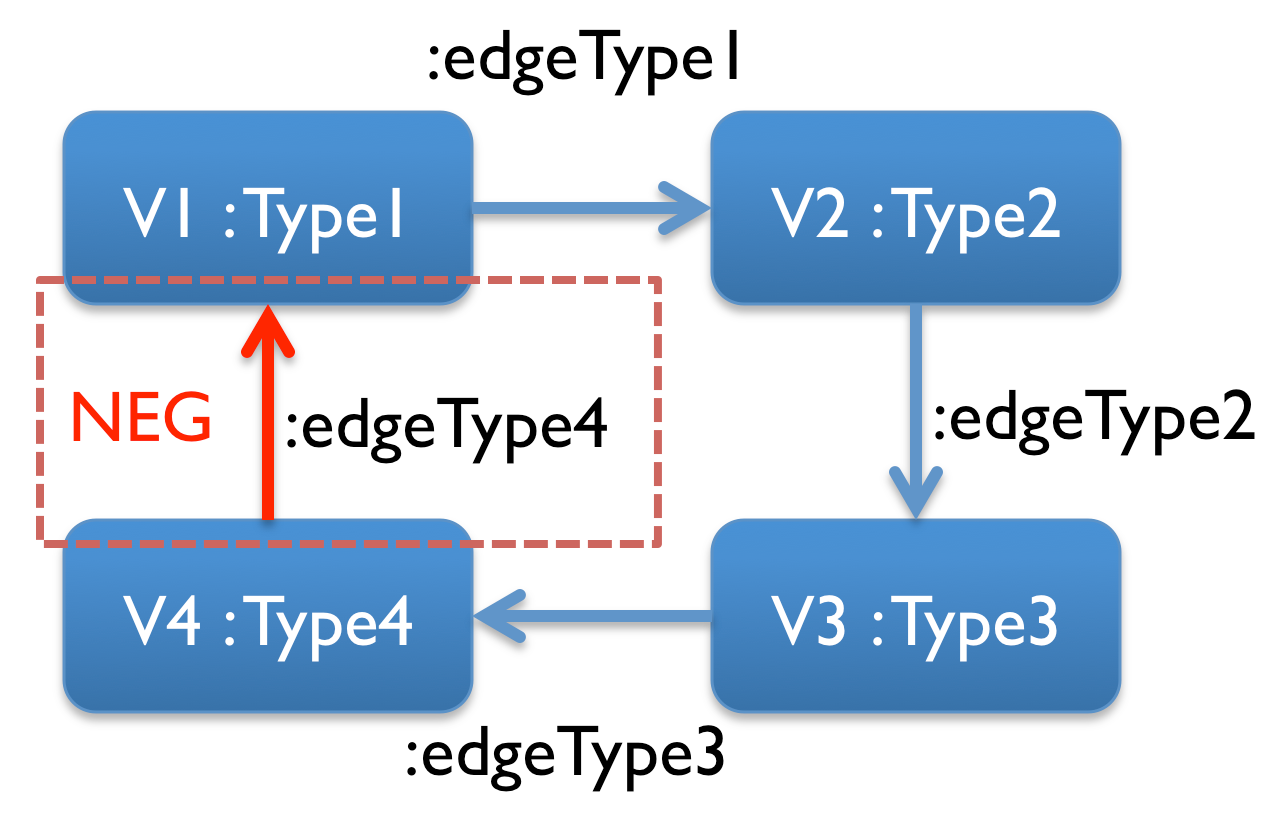
\includegraphics[width=\textwidth]{figures/patterndef}
% \end{minipage}
% \end{tabular}
% \end{center}
% \caption{Example graph query}
% \label{fig:patterndef}
% \end{figure}



\subsection{Scalability considerations}
For the storage layer, the most important issue from an incremental query evaluation perspective is that the indexers of the middleware should be filled as quickly as possible. This favors technologies where model sharding can be performed efficiently (i.e.\ with balanced shards in terms of type-instance relationships), and elementary queries (or model graph traversals) can be executed efficiently.

Achieving scalability of the distributed Rete architecture is an equally complex challenge. The overall performance of the system is influenced by a number of factors, including (i) the \emph{layout of the Rete network} (which can be optimized depending on both query and instance model characteristics, e.g.\ to keep the resource requirement of intermediate join operations to a minimum), (ii) the \emph{allocation} of Rete nodes to host computers (e.g.\ to optimize local resource usage, or to minimize the amount of remote network communication), and (iii) \emph{dynamic adaptability} to changing conditions (e.g.\ when the model size and thus query result size grows rapidly, the Rete network may require dynamic reallocation or node sharding due to local resource limitations).


\section{Deployment, configuration}
\label{sec:deployment-configuration}

Deploying, configuring and operating a distributed pattern matcher is a complex task. In the following, we will break down this task to smaller steps and present our tools for solving them. 

\subsection{Tooling}

We aimed to build \iqd{} on top of \eiq{}'s pattern language (IQPL) and its Rete net generator. For the allocation of Rete nodes, we created an Eclipse-based editor and viewer.

\subsection{Degrees of freedom}

The deployment and configuration of a distributed pattern matcher involves many degrees of freedom:

\begin{itemize}
  \item We may choose different database implementations due to the \iqd{}'s backend-agnostic nature. Until now, we experimented with property graph databases (Neo4j, Titan) and triplestores (4store).
  \item We may use different database sharding strategies (e.g.\ random partitioners or more sophisticated sharding methods based on domain-specific knowledge).
  \item We may choose diffent strategies to allocate the Rete nodes. Note that in theory, this is orthogonal to the database's sharding strategy. However, we expect that keeping the Rete network's type indexer nodes and the instances of the given type on the same server would decrease the initialization time significantly.
\end{itemize}

\subsection{Workflow}
\label{subsec:workflow}

In the following part, we will describe the workflow behind the pattern matching process. Starting from a metamodel, an instance model and a graph pattern, we will cover the problem pieces that need to be solved for setting up an incremental, distributed pattern matcher. The workflow is shown on \figref{recipe}.

\myFigureSmall{recipe}{The workflow of \eiq{} (blue) and \iqd{} (green)}

\subsubsection{Analyze the metamodel and the query}

\paragraph{Task.} First, we determine the constraints defined by the query pattern. The matches satisfying these constraints will define the results of the query.

\paragraph{Implementation.} The pattern is defined in an IQPL (\iq{} Pattern Language) text file. Using Xtext \cite{Xtext}, an Eclipse-based framework for creating domain-specific languages, the textual representation of the pattern is parsed to an EMF model. Based on the EMF model's pattern and the metamodel, a constraint network called \textit{PSystem} (short for \textit{Pattern System}) is generated. 

\subsubsection{Build a Rete layout}

\paragraph{Task.} To allow incremental query evaluation, we create a Rete net based on the constraints derived from the query.

\paragraph{Implementation.} As we mentioned earlier, we aim to reuse as much of \eiq{}'s existing code base as possible. As part of this attempt, we introduced the concept of \textit{Rete recipe}s which define the layout of a Rete network.    

\subsubsection{Allocate the Rete network in the cloud's nodes} 

\paragraph{Task.} Because of its single workstation nature, \eiq{} simply unfolds the Rete net based on the derived Rete recipe. At the same time, \iqd{} operates in a distributed environment where local resource exhaustion, network latency and throughput are critical aspects. 

\paragraph{Implementation.} Currently, the allocation of the Rete nodes is done manually. To address this limitation, we plan to utilize Constraint Satisfaction Problem (CSP) solvers, or dynamic techniques like Design Space Exploration (DSE)~\cite{DSE11}. 

\subsubsection{Bootstrap the system}

\paragraph{Task.} Based on the Rete network's allocation, we have to deply the Rete nodes in the distributed systems. After the successful deployment, the Rete network has to be initialised. Due to the Rete algorithm's asynchronous nature, it uses a termination protocol to signal when the data processing is finished. 

\paragraph{Implementation.} In \iqd{}'s prototype, both the bootstrapping and the Rete network's operation is carried out automatically. The Akka actors representing the Rete nodes are deployed and initiated using Akka's \textit{programmatic remote deployment} feature. 



\section{Elaboration of the Example}
\label{sec:elaboration}

To demonstrate \iqd{}'s approach, we elaborate an example in detail. We introduce a case study, then formulate a query and show the workflow that executes the distributed, incremental evaluation of the pattern defined by query.

\pic{trainbenchmark-metamodel}{The EMF metamodel of the railroad system}

%%%%%%%%%%%%%%%%%%%%%%%%%%%%%%%%%%%%%%%%%%%%%%%%%%%%%%%%%%%%%%%%%%%%%%%%%%%%%%%%%%%%%%%%%%%%%%%%%%%%

\subsection{Case Study: Railroad System Design}
\label{railroad-system}

\pic{neoclipse-graph}{A subgraph of a railroad system visualized}

The example is built around an imaginary railroad system. The system's network is composed of typical railroad items, including signals, segments, switches and sensors. The complete EMF metamodel is shown on \figref{trainbenchmark-metamodel}. A subgraph of an instance model is shown on \figref{neoclipse-graph}.

We defined queries that resemble a typical MDE application's workload. In general, MDE queries are more complex than those used in traditional databases. They often define large patterns with multiple join operations. The queries look for violations of \emph{well-formedness constraints} in the model. In this section, we discuss the \textit{RouteSensor} query in detail.

% TODO see more in the benchmark section?
%Although the \tb{} defines a total of four queries, in this report we only discuss the \textit{RouteSensor} query in detail.

\subsubsection{RouteSensor}

\pic{routesensor-pattern}{Graphical representation of the RouteSensor query's pattern. The dashed red arrow defines a negative application condition.}

The \textit{RouteSensor} query looks for \texttt{Sensor}s that are connected to a \texttt{Switch}, but the \texttt{Sensor} and the \texttt{Switch} are \emph{not} connected to the same \texttt{Route}. The graphical representation of the RouteSensor query is shown on \figref{routesensor-pattern}. Basically, the RouteSensor query binds the type of the vertices, defines three edges and one negative edge, called NAC (negative application condition). 


\lstset{language=viatra}

\begin{lstlisting}[caption=The RouteSensor query in IQPL, label=lst:routesensor-iqpl]
package hu.bme.mit.train.constraintcheck.incquery

import "http://www.semanticweb.org/ontologies/2011/1/TrainRequirementOntology.owl" 

pattern routeSensor(Sen, Sw, Sp, R) = {
	Route(R);
	SwitchPosition(Sp);
	Switch(Sw);
	Sensor(Sen);
	
	Route.Route_switchPosition(R, Sp);
	SwitchPosition.SwitchPosition_switch(Sp, Sw);
	Trackelement.TrackElement_sensor(Sw, Sen);
	
	neg find head(Sen, R);	
}

pattern head(Sen, R) = {
	Route.Route_routeDefinition(R, Sen);
}
\end{lstlisting}

The RouteSensor query in IQPL (\iq{} Pattern Language) %(\autoref{subsec:eiq}) 
is shown on \lstref{routesensor-iqpl}. This query binds the variables (\texttt{Sen}, \texttt{Sw}, \texttt{Sp}, \texttt{R}) to the appropriate type. It defines the three edges as relationships between the variables and defines the negative application condition as a negative pattern (\texttt{neg find}).

For comparison, we also present the RouteSensor query in SPARQL (RDF's query language) on \lstref{routesensor-sparql}. Here, the types are defined with the \texttt{rdf:type} predicate, while the edges are defined with \texttt{base} predicates. The negative application condition is defined with the \texttt{FILTER NOT EXISTS} construction\footnote{Note that the two queries are slightly different: the SPARQL query returns only a set of \texttt{Sensor}s, while the IQPL query returns a set of (\texttt{Sensor}, \texttt{Switch}, \texttt{SwitchPosition}, \texttt{Route}) tuples.}.

\lstset{language=SQL,morekeywords={PREFIX,FILTER}} %,java,rdf,rdfs,url,owl,base}}

\begin{lstlisting}[caption=The RouteSensor query in SPARQL, label=lst:routesensor-sparql]
PREFIX base: <http://www.semanticweb.org/ontologies/2011/1/TrainRequirementOntology.owl#>
PREFIX rdfs: <http://www.w3.org/2000/01/rdf-schema#>
PREFIX owl:  <http://www.w3.org/2002/07/owl#>
PREFIX rdf:  <http://www.w3.org/1999/02/22-rdf-syntax-ns#>

SELECT DISTINCT ?xSensor
WHERE
{
    ?xRoute rdf:type base:Route .
    ?xSwitchPosition rdf:type base:SwitchPosition .
    ?xSwitch rdf:type base:Switch .
    ?xSensor rdf:type base:Sensor .
    ?xRoute base:Route_switchPosition ?xSwitchPosition .
    ?xSwitchPosition base:SwitchPosition_switch ?xSwitch .
    ?xSwitch base:TrackElement_sensor ?xSensor .

    FILTER NOT EXISTS {
        ?xRoute ?Route_routeDefinition ?xSensor .
    } .
}
\end{lstlisting}

%%%%%%%%%%%%%%%%%%%%%%%%%%%%%%%%%%%%%%%%%%%%%%%%%%%%%%%%%%%%%%%%%%%%%%%%%%%%%%%%%%%%%%%%%%%%%%%%%%%%

\picSmall{recipe}{\iqd{}'s workflow} 

\subsection{Workflow of the Example}
\label{example-workflow}

Following the workflow defined in \autoref{iqd-workflow}, we will cover the steps for deploying and operating a distributed pattern matcher for the \textit{RouteSensor} query.

\subsubsection{Constructing a Rete net}

First, using \eiq{}'s tooling, the query (\texttt{routeSensor.iqpl}, see \lstref{routesensor-iqpl}) is analyzed and parsed to an EMF model %(\figref{eiq-model})
\textcircled{1}.

%\picTiny{eiq-model}{The EMF model generated from the RouteSensor query's pattern}

The metamodel (\texttt{railroad.ecore}) is shown on \figref{trainbenchmark-metamodel}. Based on the query \textcircled{2} and the metamodel \textcircled{3} \eiq{} builds a \emph{pattern system} (PSystem). The PSystem is translated to a Rete recipe, the system derives a Rete layout \textcircled{4}, that guarantees the satisfaction of the constraints. The Rete layout is shown on \figref{rete-routesensor-layout}.

\pic{rete-routesensor-layout}{The RouteSensor query's layout}

\subsubsection{Deploying the Rete Net}

The Rete nodes are allocated to the cluster's servers by providing the infrastructure mapping \textcircled{5}.

%\picTiny{incqueryd-tooling-tree-editor}{The tree editor in \iqd's tooling}

In \iqd{}'s current implementation, the Rete recipe's nodes are allocated manually on the cloud servers (called \textit{Machine}s). The Rete nodes are associated with the machines with \textit{infrastructure mapping} relationships. \iqd{}'s tooling currently provides an Eclipse-based tree editor to define machines and the infrastructure mapping edges.% (\figref{incqueryd-tooling-tree-editor}). 

The tooling is capable of visualizing the Rete network and its mapping to the machines (see \figref{incqueryd-tooling-yfiles-viewer}).
The Rete network is deployed to the Akka instances running on the servers \textcircled{6}.

\picSmall{incqueryd-tooling-yfiles-viewer}{The yFiles viewer in \iqd's tooling}

\subsubsection{Evaluating Query}

The query is evaluated by initializing the Rete net \textcircled{7} and reading the results from its production node. 
%In \iqd{}'s current implementation, the distributed system is . The Akka actors representing the Rete network's nodes are deployed automatically by the \iqd{} \textit{Coordinator} node.

\subsubsection{Maintaining the Query Results}

In order to provide query results that are consistent with the model, we need maintain the Rete net's state. Suppose we have the graph shown on the left side of \figref{rete-routesensor-example-instances-neoclipse} loaded to the Rete net and we decide to delete the \texttt{ROUTE\_ROUTEDEFINITION} edge between vertices 2 and 1.

\pic{rete-routesensor-example-instances}{A modification on a \tb{} instance model}

\figref{rete-routesensor-example-distributed} shows the distributed Rete net containing the partial matches of the original graph. When we delete the edge between vertices 2 and 1, the \texttt{ROUTE\_ROUTEDEFINITION} type indexer receives a notification from the middleware and sends a \textit{negative update} \textcircled{1} with the tuple $(2, 1)$. The antijoin node processes the negative update and propagates a negative update \textcircled{2} with the tuple $(3, 4, 2, 1)$. This is received by the production node, which initiates the \textit{termination protocol} \textcircled{3}, \textcircled{4}. After the termination protocol finishes, the indexer signals the client about the successful update. The client can now retrieve the results from the production node. The client may choose to retrieve only the ''deltas'', i.e.\ only the the tuples that have been added or deleted since the last modification.

\pic{rete-routesensor-example-distributed}{Operation sequence on a distributed Rete net}



